\documentclass{article}

\usepackage{graphicx}
\usepackage{tikz}
\usepackage{tikzsymbols}
\usetikzlibrary{calc,patterns,shapes.geometric}
\pagestyle{empty}
\usepackage[margin=0pt]{geometry}
\geometry{papersize={14in,12in}}

\def\centerarc[#1](#2)(#3:#4:#5){\draw[#1] ($(#2)+({#5*cos(#3)},{#5*sin(#3)})$) arc (#3:#4:#5);}

\begin{document}
	\begin{figure}
		\centering
		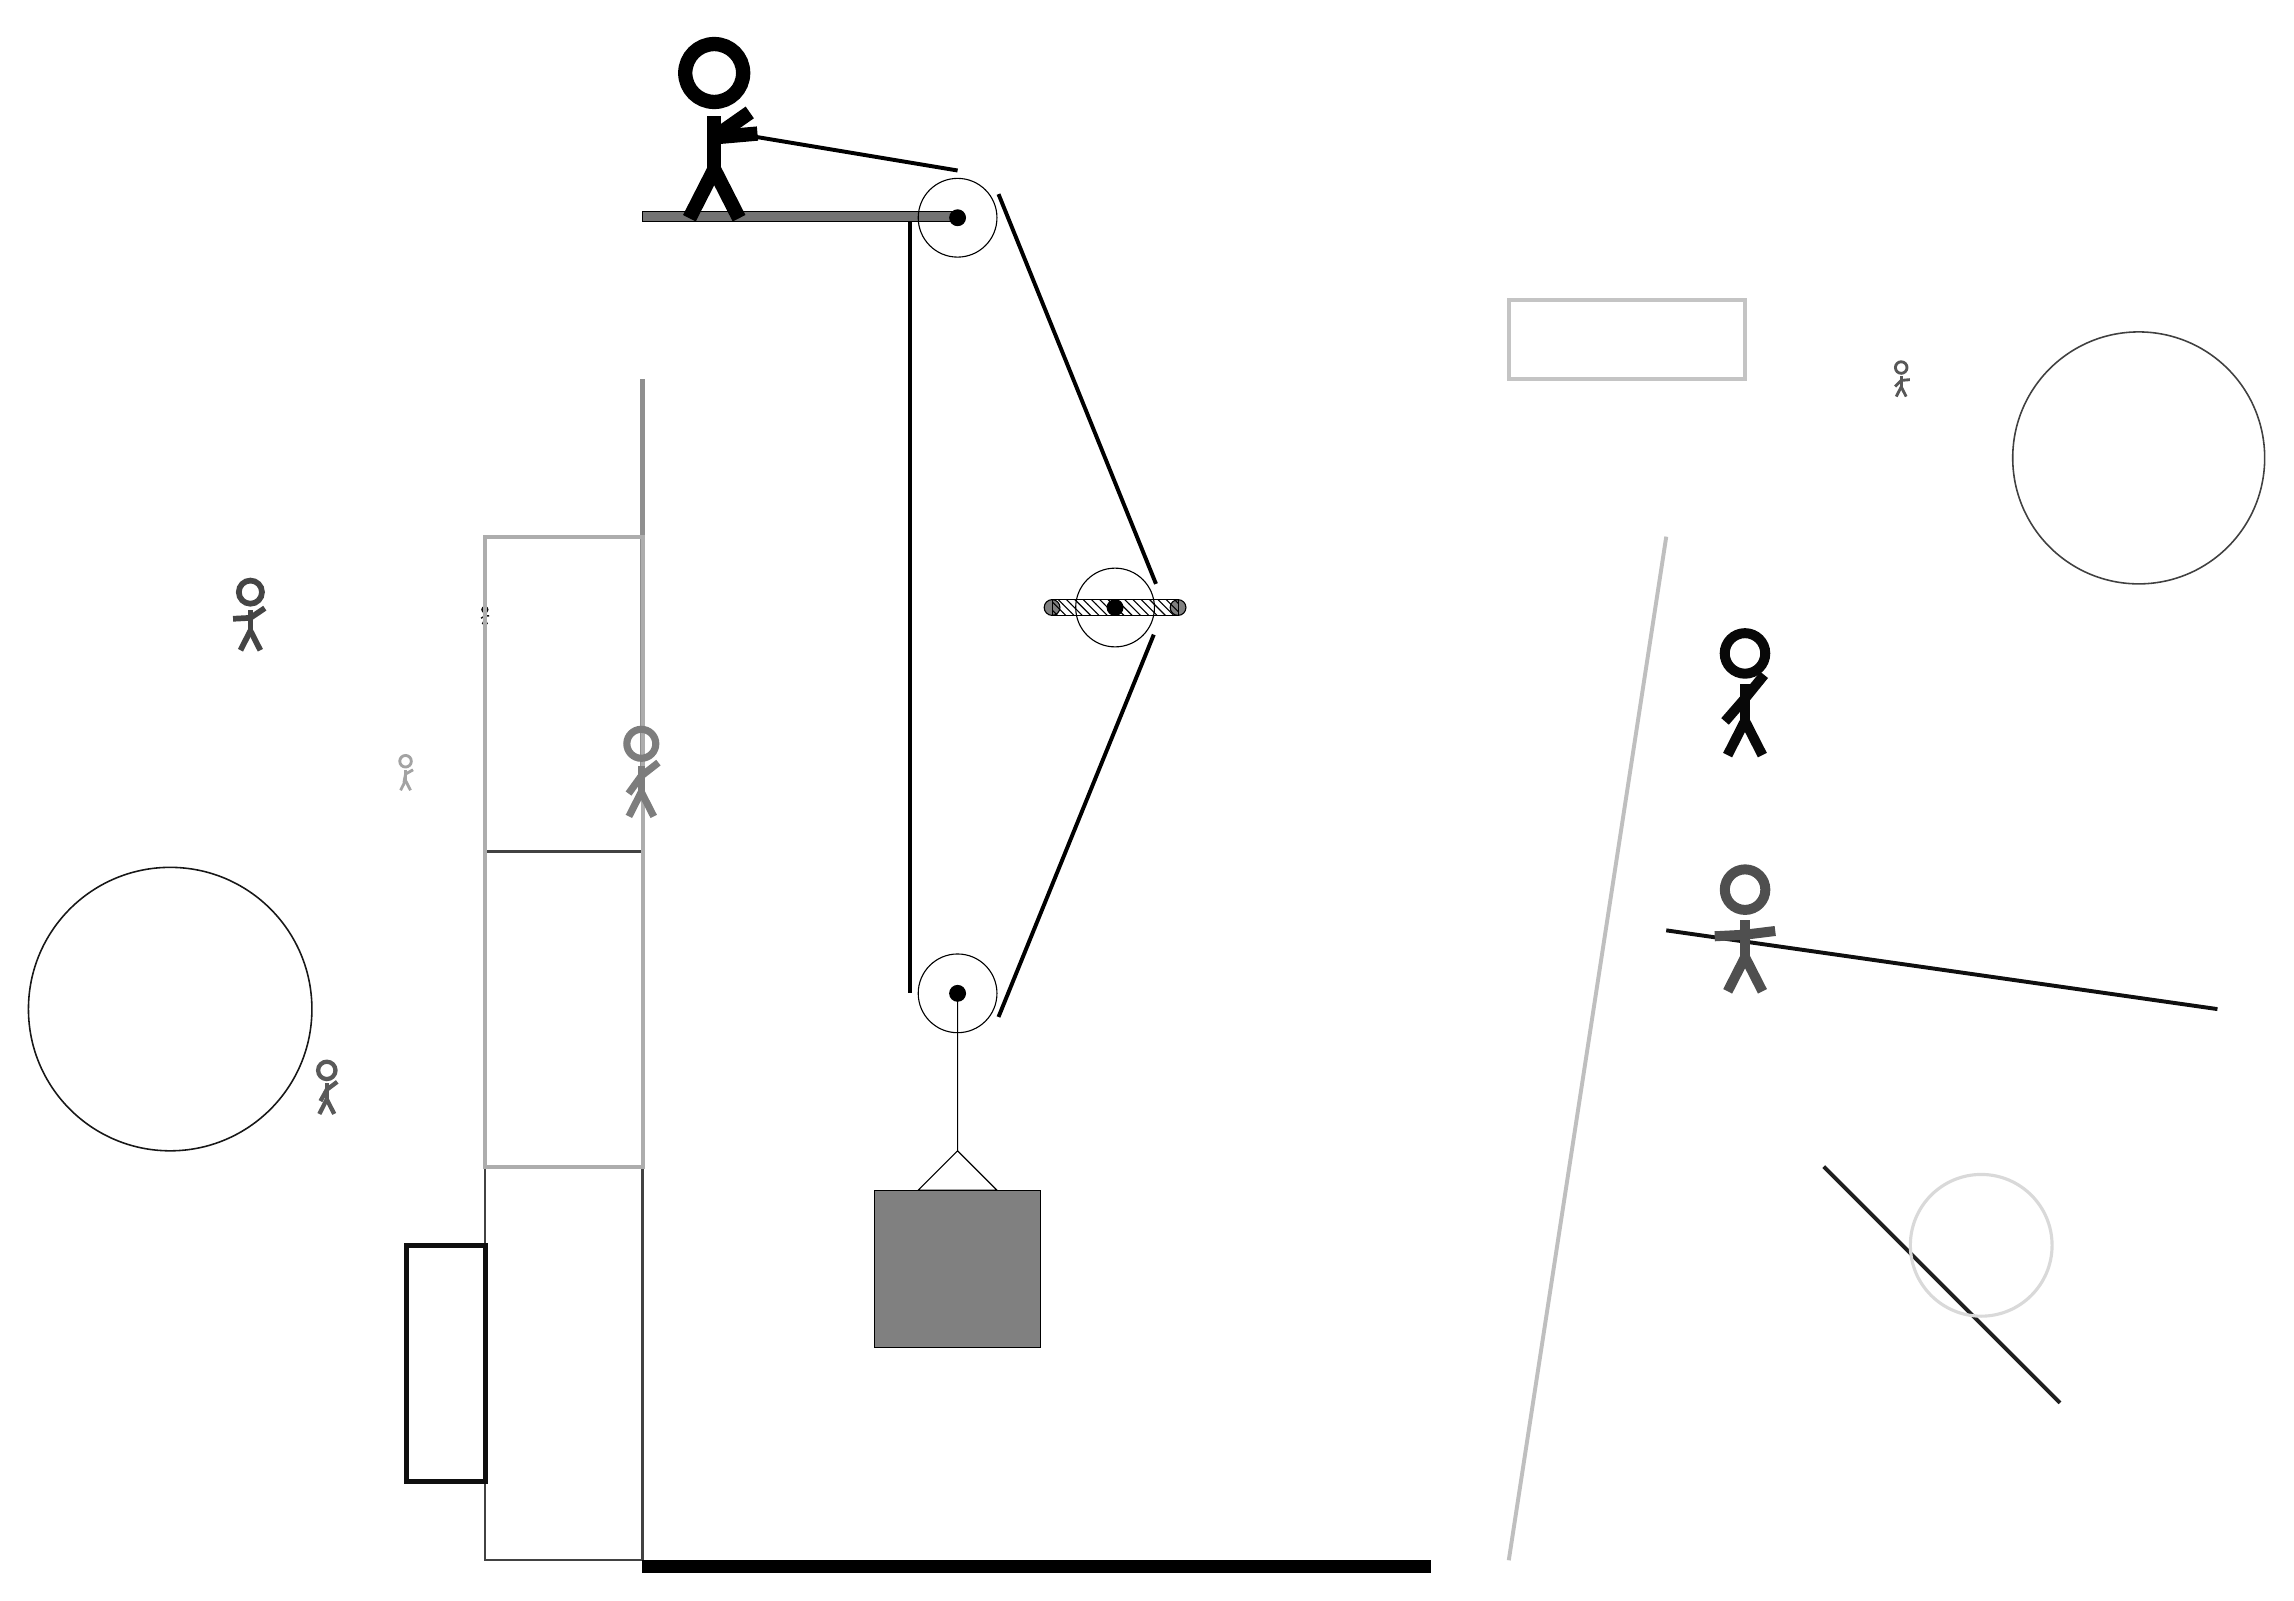
\begin{tikzpicture}
			%%%%% START %%%%%
			
			\draw[fill=black!55] (-2, 14) rectangle (2, 14.125);
			
			\node[line width=0.2mm, color=black!36] at (-5, 7) {\Strichmaxerl[2][79][30]};
			
			\node[line width=0.5mm, color=black!66] at (14, 12) {\Strichmaxerl[2][45][5]};
			\draw[line width=0.5mm, color=black!23] (9, 12) rectangle (12, 13);
			\node[line width=0.2mm, color=black!94] at (-4, 9) {\Strichmaxerl[1][30][2]};
			\draw[line width=0.5mm, color=black!94](11, 5) -- (18, 4);
			
			\draw[line width=0.3mm, color=black!74] (-2, 6) rectangle (-4, -3);
			\draw[line width=0.4mm, color=black!46] (-2, 6) rectangle (-2, 2);
			
			\node[line width=0.5mm, color=black!73] at (-7, 9) {\Strichmaxerl[4][3][34]};
			\draw [line width=0.2mm, color=black!75](17, 11) circle (1.6);
			\draw[line width=0.6mm, color=black!44] (-2, 12) rectangle (-2, 7);
			
			\draw[line width=0.5mm, color=black!32] (-4, 2) rectangle (-2, 10);
			\draw[line width=0.5mm, color=black!88](13, 2) -- (16, -1);
			\node[line width=0.3mm, color=black!97] at (12, 8) {\Strichmaxerl[7][49][51]};
			\node[line width=0.7mm, color=black!65] at (-6, 3) {\Strichmaxerl[3][61][37]};
			\draw [line width=0.4mm, color=black!15](15, 1) circle (0.9);
			\draw[line width=0.6mm, color=black!94] (-4, 1) rectangle (-5, -2);
			
			\draw[line width=0.5mm, color=black!25](11, 10) -- (9, -3);
			\draw[line width=0.5mm, color=black!47](12, 8) -- (12, 8);
			\node[line width=0.6mm, color=black!69] at (12, 5) {\Strichmaxerl[7][3][7]};
			\draw [line width=0.2mm, color=black!91](-8, 4) circle (1.8);
			\node[line width=0.2mm, color=black!51] at (-2, 7) {\Strichmaxerl[5][54][38]};
			
			
			\draw (2, 4.2) circle (0.5);
			\draw[fill=black] (2, 4.2) circle (0.1);
			
			\draw (2, 14.05) circle (0.5);
			\draw[fill=black] (2, 14.05) circle (0.1);
			
			\draw[fill=white](4, 9.1) circle (0.5);
			\draw[fill=black] (4, 9.1) circle (0.1);
			\draw[fill=black!50] (3.2, 9.1) circle (0.1);
			\draw[fill=black!50] (4.8, 9.1) circle (0.1);
			\draw[pattern=north west lines, pattern color=black] (3.2, 9.2) rectangle (4.8, 9.0);
			
			\draw (2, 4.2) -- (2, 2.2) -- (1.5, 1.7) -- (2.5, 1.7) -- (2, 2.2);
			\draw[fill=black!50] (0.95, 1.7) rectangle (3.05, -0.3);
			
			\draw[line width=0.5mm] (1.4, 14) -- (1.4, 4.2);
			\centerarc[line width=0.5mm](2, 4.2)(180:330:0.6);
			\draw[line width=0.5mm](2.5196, 3.9) -- (4.4915, 8.7558);
			\centerarc[line width=0.5mm](4, 9.1)(390:325:0.6);
			\draw[line width=0.5mm](4.5196, 9.4) -- (2.5196, 14.35);
			\centerarc[line width=0.5mm](2, 14.05)(30:90:0.6);
			\draw[line width=0.5mm](2, 14.65) -- (-1, 15.15);
			
			\node at (-1, 15.15) {\Strichmaxerl[10][-175][35]};
			
			\draw[fill=black] (-2, -3) rectangle (8, -3.15);
			
			%%%%% END %%%%%
		\end{tikzpicture}
	\end{figure}	
\end{document}